\documentclass[11pt]{article}

\usepackage{booktabs}
\usepackage{homeworkpkg}
\usepackage{enumitem}
\usepackage[font=small,labelfont=bf]{caption}
\usepackage[bottom]{footmisc}

\newlength\dunder
\settowidth{\dunder}{\_}

\graphicspath{ {images/} }

%% Local Macros and packages: add any of your own definitions here.

\begin{document}

% Homework number, your name and NetID, and optionally, the names/NetIDs of anyone you collaborated with. If you did not collaborate with anybody, leave the last parameter empty.
\homework
    {2}
    {Nestor Alejandro Bermudez Sarmiento (nab6)}
    {}

In this assignment we have implemented general-purpose search algorithms to solve well know puzzles. In the first section we'll use such algorithms to 'guide' a 'Pacman' through the maze, finding all the food pellets. In the second section we'll solve the Sokoban puzzle and describe the chosen heuristic and why it is valid.\\

We've decided to use Python for this assignment. The source code is provided with this report and will also be available under the following GitHub account right after the submission deadline had passed. See \href{https://github.com/nbermudezs/UIUC_CS440}{Nestor's GitHub CS440 repository}.\\

\section*{Part 1}

\pagebreak
\section*{Part 2: Breakthrough}
Just like in the previous assignment we will use bitmaps to represent the state of the board. Having two bitmaps, one per player, of size equals to the size of the board. A value of 1 indicates that the piece of that player is in a given position.\\

We implemented a \textbf{Game} class inspired in the code for the textbook\footnote{\url{https://github.com/aimacode/aima-python}}. The class is a simple empty skeleton that specifies which methods a game must implement. We then implemented a \textbf{Breakthrough} class that extends \textbf{Game} and implements all its methods. There is a function to generate all the possible actions for a given player given the current state of the board and, more importantly, there is a function that determines when a state is terminal. The \textbf{Breakthrough} class can handle any board size and we use it for the extended rule of using a rectangular board.\\

For the game with the extended rule to take 3 workers home we created a new class called \textbf{Breakthrough3WorkersToBase} which inherits everything from the previous \textbf{Breakthrough} class but overrides the \textit{terminal\_test} function.\\

From now on whenever we may refer to the \textit{state} as the \textit{board} and vice versa. Note that the board has been implemented as a class called \textbf{BreakthroughBoard} and it is responsible of actually moving the pieces/capturing based on an original and final position.


\subsubsection*{Heuristic}
All the heuristic functions can be found under the \textbf{Heuristics} class. Each of the methods is expected to receive two arguments, the first one is the game instance and the second one is the current state. \\

The implementation of the two given heuristics is rather simple. For \textbf{Defensive 1} we simply count how many ones are in the corresponding bitmap of our state representation. Once we have the count we just apply the formula provided. The same goes for \textbf{Offensive 1} with the only difference that you need to look at the other bitmap. \\

For \textbf{Defensive 2} we implemented a weighted function that considers these features of the board:
\begin{enumerate}
\item number of protected cells (both ours and the opponent's): this is the number of cells that can be reached from one of the pieces in a single move and that are not occupied by another piece.
\item row formations: this is when at least two pieces are next to each other.
\item delta formations: this is when a given piece has two pieces diagonally behind it.
\item base cells: how many pieces are still in their base. We value this because they are our last line of defense.
\end{enumerate}

We played a little bit with the weight of each of the features and we ended up with the best results when:
\begin{enumerate}
\item the score is punished for each unprotected cell. An unprotected cell is one that is under attack by the opponent but is it defended by one of your own pieces. For each of those cells we reduce our score by 100.
\item for each of the delta formations we add 75 points to our board score and reduce 75 for each enemy delta formation. We value these formations this high because if a piece is captured we can always retaliate. 
\item protected cells add 65 points each. Cells protected by the enemy reduces 65 points.
\end{enumerate}

Besides those features we also check for pieces that are about to win, on both sides, and add or subtract from the score accordingly.\\

For \textbf{Offensive 2} we also implemented a weighted function of features. These are the features:
\begin{enumerate}
\item proximity to the goal: how far into the enemy territory a piece is.
\item arrow formations: created by a piece and all the cells behind it being occupied by friendly pieces.
\item almost win position: increase or decrease the score if board can be won/lost on the next move.
\end{enumerate}

Just like for \textbf{Defensive 2} we played with the weights and settled with:
\begin{enumerate}
\item proximity: 5 points for each row closer to the goal
\item arrow formation: 20 points
\item almost win/lose: 1000 points
\end{enumerate}

\subsubsection*{Analysis}
Why \textbf{Defensive 2} works?\\
Our heuristic emphasizes coverage of the board and delta formations; since \textbf{Offensive 1} only depends on the remaining enemy pieces it is expected that it will try to capture whenever possible. This will immediately be punished if there is a delta formation unless it is about to win. Also, since we value protected cells, we will have more opportunities to capture a piece if it treating us.\\

Why \textbf{Offensive 2} works?\\
Note that our heuristic does not weight in the number of pieces on either side, this offensive strategy relies to getting as far without necessarily capturing pieces, this should allow us to reduce the change of triggering a response from \textbf{Defensive 1}.\\

\subsubsection*{Results 2.1}
For each of the match-ups requested we played the game four times. The averages are shown below but the results for the individual match-ups can be found in the summary spreadsheet delivered with this report and also online\footnote{\url{https://docs.google.com/a/illinois.edu/spreadsheets/d/1304kvtHACh1N3kYYjGNfJnYtcIc5_p1jHPop4sn356I/edit?usp=sharing}}.\\
In the zip file accompanying this report you will find the whole sequence of moves for every game summarized in this report, as well as the stats for each player. See the \textit{results} directory.\\
Any time measurement is assumed to be in seconds.\\

\textbf{1. Minimax (Offensive 1) vs Alpha-beta (Offensive 1)}\\
Minimax used depth 4 and Alpha-beta used depth 5.
Game results:
\begin{enumerate}
\item Average time per move for whites: \textbf{16.03}
\item Average time per move for blacks: \textbf{0.91}
\item Average \# nodes expanded per move for whites: \textbf{413,445.82}
\item Average \# nodes expanded per move for blacks:  \textbf{21,177.43}
\item Total \# nodes expanded by whites: \textbf{2,796,884.5}
\item Total \# nodes expanded by blacks: \textbf{143,064}
\item Total \# of moves: \textbf{13.5}
\item White pieces captured: \textbf{0.25}
\item Black pieces captured: \textbf{1.5}
\item Winner: Whites
\end{enumerate}
\begin{center}
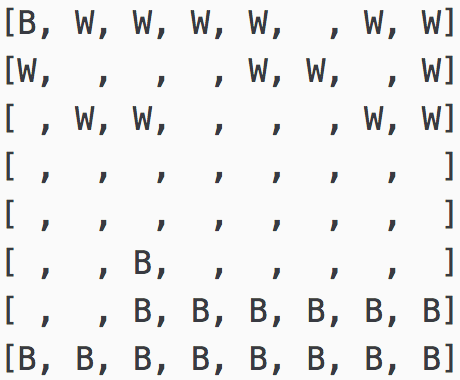
\includegraphics[scale=1]{part2/minimax-o1-vs-ab-o1.png}\\
Final state of the board.
\end{center}
Trends: in all the games the Alpha-beta player won. Which makes since it can see one more move ahead. \\

\pagebreak
\textbf{2. Alpha-beta (Offensive 2) vs Alpha-beta (Defensive 1)}\\
This was run with depth of 4 for both players.\\
Game results:\\
\begin{enumerate}
\item Average time per move for whites: \textbf{0.66}
\item Average time per move for blacks: \textbf{0.25}
\item Average \# nodes expanded per move for whites: \textbf{7,544.1}
\item Average \# nodes expanded per move for blacks:  \textbf{4,403.9}
\item Total \# nodes expanded by whites: \textbf{189,886.75}
\item Total \# nodes expanded by blacks: \textbf{102,276.5}
\item Total \# of moves: \textbf{49.5}
\item White pieces captured: \textbf{0}
\item Black pieces captured: \textbf{2.75}
\item Winner: Whites
\end{enumerate}
\begin{center}
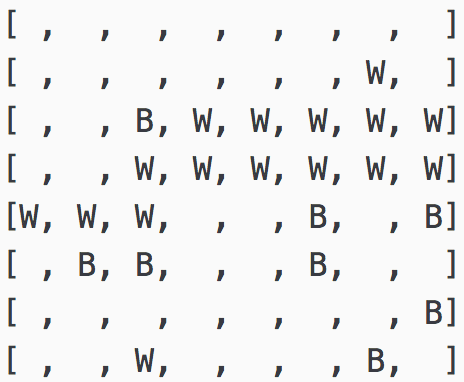
\includegraphics[scale=1]{part2/ab-o2-vs-ab-d1.png}\\
Final state of the board.
\end{center}
Trends: Our heuristic won 3 out of the 4 games played. It was nice to see that the formation that we intended to see in the board actually appeared. Here is an example: \\
\begin{center}
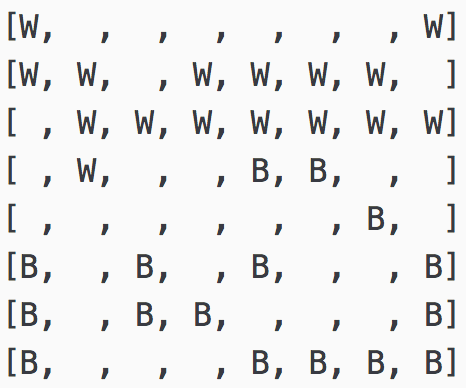
\includegraphics[scale=1]{part2/ab-o2-vs-ab-d1-pattern.png}
\end{center}
See how the white pieces advance but don't try to go on their own and always have "backup".\\

\pagebreak
\textbf{3. Alpha-beta (Defensive 2) vs Alpha-beta (Offensive 1)}\\
This was run with depth of 4 for both players.\\
Game results:\\
\begin{enumerate}
\item Average time per move for whites: \textbf{55.39}
\item Average time per move for blacks: \textbf{3.34}
\item Average \# nodes expanded per move for whites: \textbf{10,067.28}
\item Average \# nodes expanded per move for blacks:  \textbf{2,514.29}
\item Total \# nodes expanded by whites: \textbf{160,601.75}
\item Total \# nodes expanded by blacks: \textbf{45,653.75}
\item Total \# of moves: \textbf{36}
\item White pieces captured: \textbf{0}
\item Black pieces captured: \textbf{2}
\item Winner: Whites
\end{enumerate}
\begin{center}
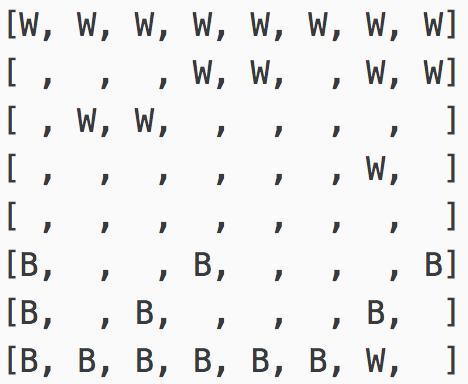
\includegraphics[scale=1]{part2/ab-d2-vs-ab-o1.png}\\
Final state of the board.
\end{center}
Trends: Our heuristic won 4 out of the 4 games played. The delta formations we were expecting to see showed up most of the times. Here is an example: \\
\begin{center}
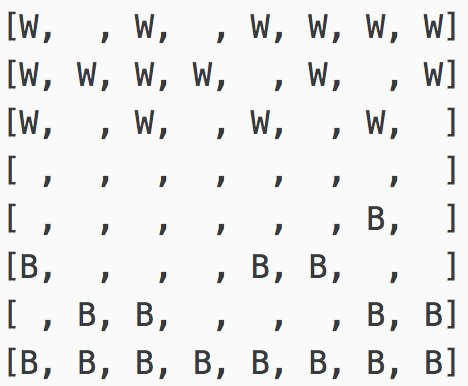
\includegraphics[scale=1]{part2/ab-d2-vs-ab-o1-pattern.png}
\end{center}
We realize this formation would be bad for a smarter opponent (and it is confirmed later on in this report) because of the "holes" in the delta formation but it turns out to work well against the provided defensive heuristic.\\

One thing to note is that for this match-up the second game took way longer than the other games. Time between moves was around 2 minutes. Our only guess is that it was caused by the fact that we were running a script for our data mining course at the same time. We could never replicate it after that.\\

\pagebreak
\textbf{4. Alpha-beta (Offensive 2) vs Alpha-beta (Offensive 1)}\\
This was run with depth of 4 for both players.\\
Game results:\\
\begin{enumerate}
\item Average time per move for whites: \textbf{0.51}
\item Average time per move for blacks: \textbf{0.17}
\item Average \# nodes expanded per move for whites: \textbf{6,463.52}
\item Average \# nodes expanded per move for blacks:  \textbf{3,183.71}
\item Total \# nodes expanded by whites: \textbf{197,461.5}
\item Total \# nodes expanded by blacks: \textbf{95,030.75}
\item Total \# of moves: \textbf{60.25}
\item White pieces captured: \textbf{0.25}
\item Black pieces captured: \textbf{4.75}
\item Winner: Whites
\end{enumerate}
\begin{center}
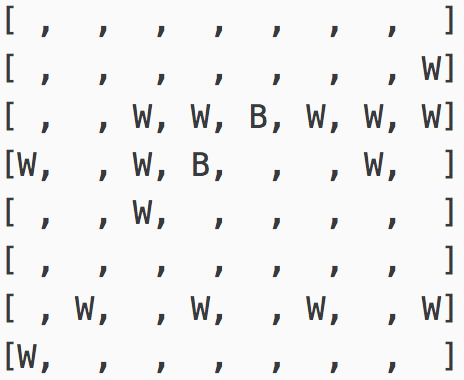
\includegraphics[scale=1]{part2/ab-o2-vs-ab-o1.png}\\
Final state of the board.
\end{center}
Trends: at first we didn't expect \textbf{Offensive 2} to beat \textbf{Offensive 1} but after looking at the results it does make sense. The reason is that almost always when \textbf{Offensive 1} would take a piece the opponent would have a way to respond because of the value we gave to "moving as a front". As a result of this, this match-up has the highest number of pieces captured on average.\\

\pagebreak
\textbf{5. Alpha-beta (Defensive 2) vs Alpha-beta (Defensive 1)}\\
This was run with depth of 4 for both players.\\
Game results:\\
\begin{enumerate}
\item Average time per move for whites: \textbf{1}
\item Average time per move for blacks: \textbf{0.22}
\item Average \# nodes expanded per move for whites: \textbf{6,111.88}
\item Average \# nodes expanded per move for blacks:  \textbf{3,524.07}
\item Total \# nodes expanded by whites: \textbf{136,086.25}
\item Total \# nodes expanded by blacks: \textbf{69,990.5}
\item Total \# of moves: \textbf{41.5}
\item White pieces captured: \textbf{0}
\item Black pieces captured: \textbf{2}
\item Winner: Whites
\end{enumerate}
\begin{center}
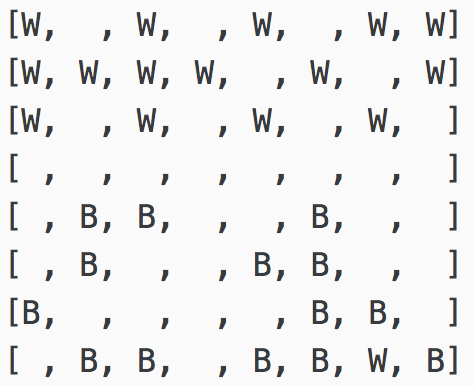
\includegraphics[scale=1]{part2/ab-d2-vs-ab-d1.png}\\
Final state of the board.
\end{center}
Trends: It makes sense for heuristic \textbf{Defensive 2} to beat \textbf{Defensive 1} because our heuristic still considers the value of the pieces as \textbf{Defensive 1} does but it also considers other features of the board.\\

\pagebreak
\textbf{6. Alpha-beta (Offensive 2) vs Alpha-beta (Defensive 2)}\\
This was run with depth of 4 for both players.\\
Game results:\\
\begin{enumerate}
\item Average time per move for whites: \textbf{0.41}
\item Average time per move for blacks: \textbf{0.22}
\item Average \# nodes expanded per move for whites: \textbf{6,010.24}
\item Average \# nodes expanded per move for blacks:  \textbf{1,680.6}
\item Total \# nodes expanded by whites: \textbf{294,502}
\item Total \# nodes expanded by blacks: \textbf{80,669}
\item Total \# of moves: \textbf{97}
\item White pieces captured: \textbf{1}
\item Black pieces captured: \textbf{14}
\item Winner: Whites
\end{enumerate}
\begin{center}
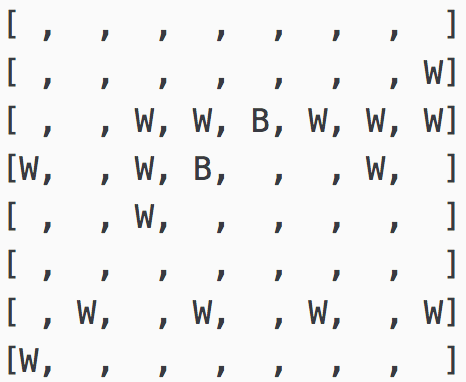
\includegraphics[scale=1]{part2/ab-o2-vs-ab-d2.png}\\
Final state of the board.
\end{center}
Trends: as mentioned earlier, \textbf{Defensive 2} heuristic isn't very smart because the delta formations leave an open path for the enemy.\\
Although we ran the match-up four times, the results were the same. This makes sense because there is no randomness on either side of the board. \\

\subsubsection*{Extended rules}
For part 2.2 we were asked to add additional rules to the board. All the code was written thinking about these extended rules since the beginning so in order to play a match in a 10x5 board the only thing we needed to do was to change the size of the board argument in our \textbf{Breakthrough} class.\\
For the 3 workers to base rule we created a new class (\textbf{Breakthrough3WorkersToBase}) that extends the normal \textbf{Breakthrough} class and overrides the \textit{terminal\_test} method.\\

Lets look at the results.\\

\subsubsection*{Results 2.2}

\textbf{1. 3 workers to base}\\
We decided to use \textbf{Offensive 1} and \textbf{Defensive 1} for the match-ups.\\

The games were run with depth of 5 for both players.\\
Game results:\\
\begin{enumerate}
\item Average time per move for whites: \textbf{3.21}
\item Average time per move for blacks: \textbf{3.1}
\item Average \# nodes expanded per move for whites: \textbf{83,946.52}
\item Average \# nodes expanded per move for blacks:  \textbf{70,858.69}
\item Total \# nodes expanded by whites: \textbf{3,938,242.75}
\item Total \# nodes expanded by blacks: \textbf{3,304,344.7}
\item Total \# of moves: \textbf{94.75}
\item White pieces captured: \textbf{7.75}
\item Black pieces captured: \textbf{9}
\item Winner: Blacks (3 out of 4 times)
\end{enumerate}
\begin{center}
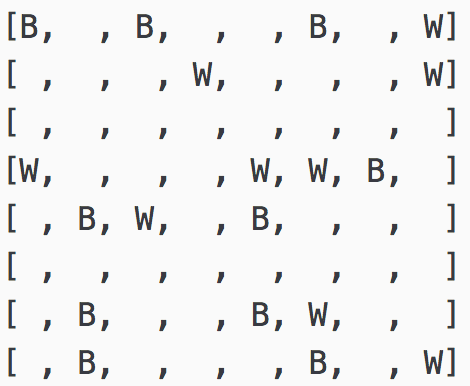
\includegraphics[scale=1]{part2/ab-o1-vs-ab-d1-3workers-black.png}\\
Game won by 3 pieces at the base.\\

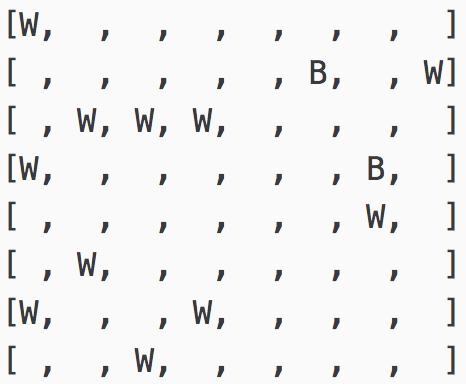
\includegraphics[scale=1]{part2/ab-o1-vs-ab-d1-3workers-whites.png}\\
Game won by 3 pieces at the base.\\
\end{center}
One of the interesting things about this setup is that the only time Whites won was because they captured all black pieces not because they took 3 pieces to base. In contrast, all the games won by Blacks were won by taking 3 pieces to base and not by capturing all white pieces. In all cases, it seems like the player that captured the most pieces wins.\\

\textbf{2. Rectangular board}\\
The games were run with depth of 5 for both players.\\
Game results:\\
\begin{enumerate}
\item Average time per move for whites: \textbf{0.86}
\item Average time per move for blacks: \textbf{0.58}
\item Average \# nodes expanded per move for whites: \textbf{23,419.22}
\item Average \# nodes expanded per move for blacks:  \textbf{14,520.39}
\item Total \# nodes expanded by whites: \textbf{760,800.25}
\item Total \# nodes expanded by blacks: \textbf{459,584}
\item Total \# of moves: \textbf{65.5}
\item White pieces captured: \textbf{1.75}
\item Black pieces captured: \textbf{6.25}
\item Winner: Whites
\end{enumerate}
\begin{center}
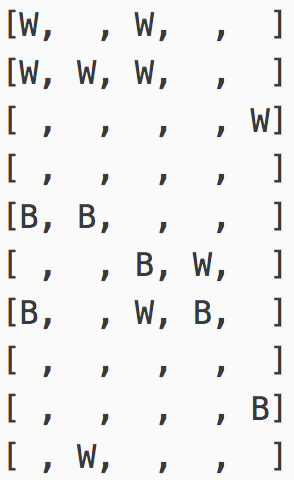
\includegraphics[scale=1]{part2/ab-o1-vs-ab-d1-rect10x5.png}\\
Final state of the board for one of the matches.
\end{center}

\subsubsection*{Potential Extra Credits}
As you may have noticed the number of expanded nodes for matches between both alpha-beta players are relatively low. We implemented move ordering based on the board configuration at depth 1. We also tried to do the ordering  on each level (inside the min-value and max-value functions) but it was taking too long to finish so we decided to keep it just in the first level.\\

We found in the book a method called \textit{beam search} which consists of just cutting off some of the search. It relies on a strong move ordering heuristic. Since our games were not taking too long we decided not to implement it. May be worth it if we increase the depth of the search to a point where we can't tolerate to consider all the actions even with alpha-beta pruning. We will try this if time permits.\\

We also ran some games in a rectangular 10x5 (as opposed to 5x10). The results were this:
\begin{enumerate}
\item Average time per move for whites: \textbf{3.08}
\item Average time per move for blacks: \textbf{1.02}
\item Average \# nodes expanded per move for whites: \textbf{79,968.26}
\item Average \# nodes expanded per move for blacks:  \textbf{24,608.09}
\item Total \# nodes expanded by whites: \textbf{1,329,205}
\item Total \# nodes expanded by blacks: \textbf{317,786.25}
\item Total \# of moves: \textbf{38.75}
\item White pieces captured: \textbf{4.5}
\item Black pieces captured: \textbf{14}
\item Winner: Whites (3 out of 4 times)
\end{enumerate}
\begin{center}
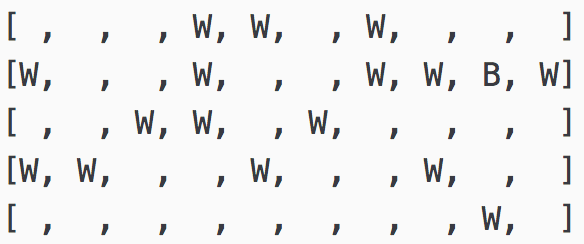
\includegraphics[scale=1]{part2/ab-01-vs-ab-d1-rect5x10.png}\\
Final state of the board for one of the matches.
\end{center}
The interesting thing about this board is that it caused the players to "think more", pretty much all the metrics are higher in this board than in the 5x10 board. This may be simply due to the fact that there are twice as many pieces which means that the number of actions at each move is higher.

\end{document}
